\documentclass[etd,oneside,senior]{BYUPhys}
\graphicspath{{./figures}}
\DeclareMathOperator{\J}{J}
\DeclareMathOperator{\struveh}{H}

% Hypergeometric function command (from https://tex.stackexchange.com/a/2477)
\newcommand*\pFqskip{8mu}
\catcode`,\active
\newcommand*\pFq{\begingroup
        \catcode`\,\active
        \def ,{\mskip\pFqskip\relax}%
        \dopFq
}
\catcode`\,12
\def\dopFq#1#2#3#4#5{%
        {}_{#1}F_{#2}\biggl[\genfrac..{0pt}{}{#3}{#4};#5\biggr]%
        \endgroup
}

% If you'd like to print your thesis using double-sided printing,
% remove the etd option and change the oneside argument to twoside, like this:
%
%\documentclass[twoside,masters]{BYUPhys}

% Your name
  \Author{Michael Greenburg}

% Enter the year your thesis is approved (for senior thesis or capstone)
  \Year{2024}

% If you have a long title, split it between multiple lines using the \\ command
  \Title{Title: Titles Must Be in Mixed Case and May Not Exceed Six Inches on One Line\\
  and Must Be in the Inverted Pyramid Format When\\
  Additional Lines Are Needed
  }

% Your research advisor
\AdvisorTitle{Advisors}
  \Advisor{Steven Turley}

% The text of your abstract
  \Abstract{The abstract is a summary of the thesis/dissertation
  with emphasis on the findings of the study. The abstract must not
  exceed 350 words in length and fit on one page, single spaced.
  
  Comptational optics things. Didn't work, no ideas on how to make it work :/}

 \Keywords{mirror, reflect}

% Acknowledge those who helped and supported you
  \Acknowledgments{
    Acknowledgements should be simple, in good taste, and fit on one page
  }

%% The members of your committee (masters only need A and B, PhD need all 4)
%  \MemberA{Committee Member A}
%  \MemberB{Committee Member B}
%  \MemberC{Committee Member C}
%  \MemberD{Committee Member D}
%

\begin{document}

% Start page counting in roman numerals
\frontmatter

% This command makes the formal preliminary pages.
% You can comment it out during the drafting process if you want to save paper.
\makepreliminarypages

% Make the table of contents.
\tableofcontents

% Start regular page counting at page 1
\mainmatter





% INTRO %%%%%%%%%%%%%%%%%%%%%%%%%%%%%%%%%%%%%%%%%%%%%%%%%%%%%%%%%%%%%%%%%%%%%%%%%%%%%%%%%%%%%%%%%%%%%%%%%%%%%%%%%%%%%%%%

\chapter{Introduction} \label{chap:intro}

\section{The Problem} \label{sec:problem}

We don't have good models of how roughness affects reflectance (CITE). There's stuff that does well when the roughness is a lot bigger or smaller than the wavelength of incident light (CITE both); this is meant to fit between.



\section{The Attempted Solution} \label{sec:attempted_solution}

Made a computational model for circular rough mirrors. It's available on \href{https://github.com/mjg0/Mirrors.jl}{GitHub}.

%%%%%%%%%%%%%%%%%%%%%%%%%%%%%%%%%%%%%%%%%%%%%%%%%%%%%%%%%%%%%%%%%%%%%%%%%%%%%%%%%%%%%%%%%%%%%%%%%%%%%%%%%%%%%%%%%%%%%%%%





% MATH %%%%%%%%%%%%%%%%%%%%%%%%%%%%%%%%%%%%%%%%%%%%%%%%%%%%%%%%%%%%%%%%%%%%%%%%%%%%%%%%%%%%%%%%%%%%%%%%%%%%%%%%%%%%%%%%%

\chapter{The Math} \label{chap:math}

\section{Expected Results} \label{sec:expected_results}

We need to make sure that our results make sense--does our program predict correct reflectance even for a flat mirror? So we need to figure out an equation that gives us what we expect: given an incident angle, $\alpha$, how would an ideal mirror react? In the far field, what is the intesity (as predicted by physical optics) at a certain polar and azimuthal angle?

\subsection{Huygens Approximation} \label{subsec:huygens_approx}

We obviously need an expected reflectance profile to make sure that what we're doing looks right. Since a flat, finite, perfectly conductive mirror is just the reflective version of an aperture (CITE), we can use the Huygen-Fresnel principle to see how light should behave when it hits a perfectly flat, perfectly reflective mirror.

Unfortunately I couldn't find an equation for diffraction through a \textit{tilted} circular aperture so I had to figure it out myself. An easy test of what I found is ensuring that whatever I come up with is identical to the circular aperture diffraction when the light comes in normal to the mirror, which is proportional to (CITE):

\begin{equation}\label{eq:airy}
  \frac{\J_1(kR\sin(\theta))}{kR\sin(\theta)}
\end{equation}

\ldots where $k$ is the wave number, $\frac{2\pi}{\lambda}$ ($\lambda$ being the wavelength), $R$ is the radius of the aperture (mirror in our case), and $\theta$ is the angle at which the reflectance is measured. $J_1$ is the first order Bessel function of the first kind. This is the Airy pattern (CITE?).

\subsubsection{Setup}

The electric field on a flat mirror in the x-y plane due to a plane wave coming in at an angle $\alpha$ from normal (the z axis), inclined toward the x axis, is proportional to (CITE?):

\begin{equation}
  e^{ikx\sin\left({\alpha}\right)}
\end{equation}

The contribution of one point on the mirror to the far field reflectance at some polar angle $\theta$ and azimuthal angle $\phi$ is just going to be that exponential multiplied by some phase shift.

\subsubsection{Phase Shift}
Since we're concerned with reflectance in the far field, all we need to determine is the phase shift relative to the origin. For some point $p$, we need to calculate the distance $d$ between that point and the origin \textit{along the direction of travel toward the point in the far field} defined by $\theta$ and $\phi$.

\begin{figure}
  \centerline{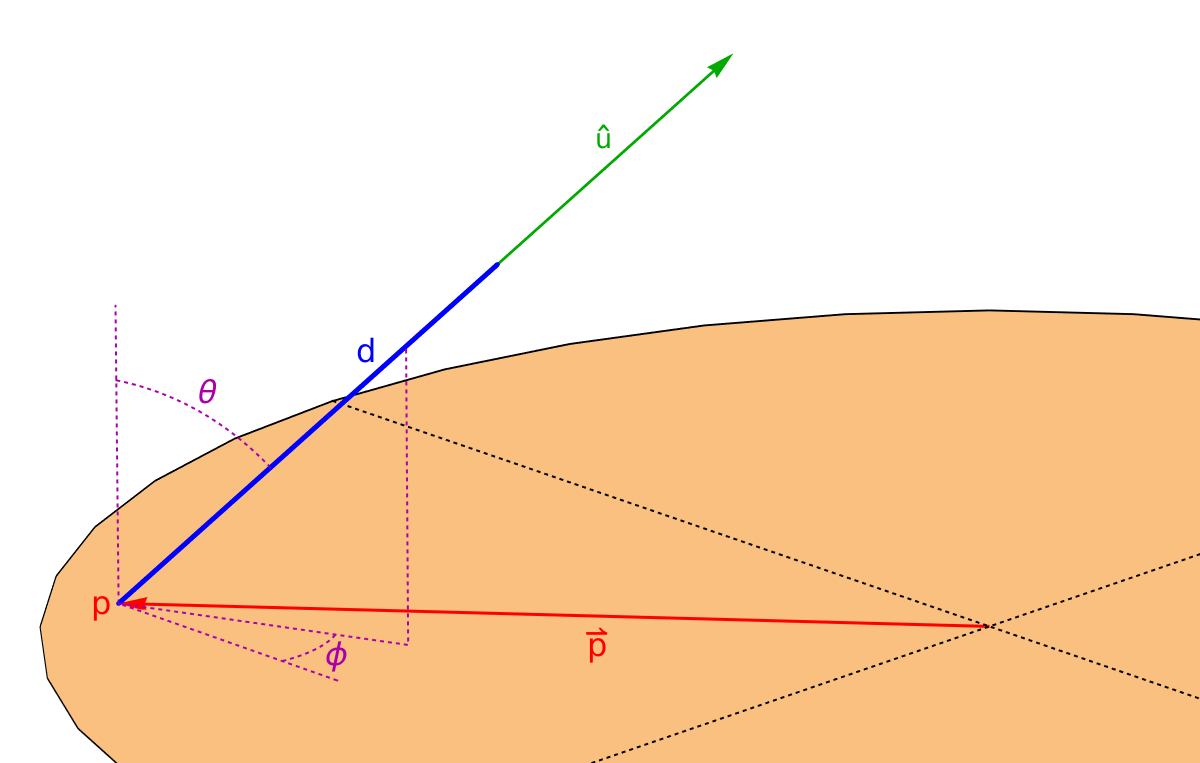
\includegraphics[width=\textwidth]{phase-length}}
  \caption[Phase length of a beam of light]{\label{fig:phase_length}
    $d$ is the phase shift of light coming from $p$ relative to light coming from the origin.}
\end{figure}

$d$ is given by dotting the unit vector $\hat{u}$ with $-\vec{p}$ [\ref{fig:phase_length}]. $\hat{u}$ is $\left(\sin{\theta}\cos{\phi},\sin{\theta}\sin{\phi},\cos{\theta}\right)$, so $d$ is:

\begin{equation}
  -x_p\sin{\theta}\cos{\phi}-y_p\sin{\theta}\sin{\phi}
\end{equation}

\ldots where $x_p$ and $y_p$ are the $x$ and $y$ coordinates of $p$.

The corresponding phase shift is thus:

\begin{equation}
  e^{-ik(x_p\sin{\theta}\cos{\phi}+y_p\sin{\theta}\sin{\phi})}
\end{equation}

\ldots so the contribution to the far field by a given point is:

\begin{equation}
  e^{ikx\sin\left({\alpha}\right)}e^{-ik(x_p\sin{\theta}\cos{\phi}+y_p\sin{\theta}\sin{\phi})}
\end{equation}

\ldots or:

\begin{equation}
  e^{ik\left(x_p(\sin{\alpha}-\sin{\theta}\cos{\phi})-y_p\sin{\theta}\sin{\phi}\right)}
\end{equation}

For simplicity, we'll define $a$ and $b$ as:

\begin{equation}
  a = k\left(\sin{\alpha}-\sin{\theta}\cos{\phi}\right)
\end{equation}
\begin{equation}
  b = -k\sin{\theta}\sin{\phi}
\end{equation}

\ldots so that we can represent the contribution from $p$ the far field as:

\begin{equation}
  e^{i(ax_p+by_p)}
\end{equation}

\subsubsection{Integrating}
To find the total contribution to the far field from the entire mirror (of radius $R$) at some $\theta$ and $\phi$, we need to integrate this contribution over the entire surface:

\begin{equation}\label{eq:integral1}
  \int_0^{2\pi}\int_0^R e^{i(ar\cos(\Theta)+br\sin(\Theta))} rdrd\Theta
\end{equation}

\ldots where I subbed in $r\cos\Theta$ and $r\sin\Theta$ for $x$ and $y$ respectively.

Due to my weak math skills, I used Mathematica to integrate this [\ref{chap:integral}]. Turns out the solution is:

\begin{equation}\label{eq:expected_refl}
  \pi R^2 \pFq{0}{1}{}{2}{-\frac{R^2}{4}\left(a^2+b^2\right)}
\end{equation}

\ldots where ${}_0 F_1$ is the confluent hypergeometric limit function. Subbing $a$ and $b$ back in appropriately, and using $\frac{2\pi}{\lambda}$ in $k$'s stead, we get:

\begin{equation}
  \pi R^2 \pFq{0}{1}{}{2}{-\frac{\pi^2 R^2}{\lambda^2}\left(\sin^2\alpha+\sin^2\theta-2\sin\alpha\sin\theta\cos\phi\right)}
\end{equation}

As a quick check, when $\alpha$ is 0 (indicating normal incident light), this is proportional to equation \ref{eq:airy} as it should be [\ref{chap:airy_validation}].

%%%%%%%%%%%%%%%%%%%%%%%%%%%%%%%%%%%%%%%%%%%%%%%%%%%%%%%%%%%%%%%%%%%%%%%%%%%%%%%%%%%%%%%%%%%%%%%%%%%%%%%%%%%%%%%%%%%%%%%%





% CODE %%%%%%%%%%%%%%%%%%%%%%%%%%%%%%%%%%%%%%%%%%%%%%%%%%%%%%%%%%%%%%%%%%%%%%%%%%%%%%%%%%%%%%%%%%%%%%%%%%%%%%%%%%%%%%%%%

\chapter{The Code}\label{chap:code} % or maybe this should just be a subsection of "Methods"

Talk about what the code does.

Talk about tests that validate that it should work.

%%%%%%%%%%%%%%%%%%%%%%%%%%%%%%%%%%%%%%%%%%%%%%%%%%%%%%%%%%%%%%%%%%%%%%%%%%%%%%%%%%%%%%%%%%%%%%%%%%%%%%%%%%%%%%%%%%%%%%%%





% APPENDICES %%%%%%%%%%%%%%%%%%%%%%%%%%%%%%%%%%%%%%%%%%%%%%%%%%%%%%%%%%%%%%%%%%%%%%%%%%%%%%%%%%%%%%%%%%%%%%%%%%%%%%%%%%%

\begin{appendices}

  \chapter{The Code}\label{chap:julia}
  
  This is where the code will be pasted in, to have some redundancy in case GitHub dies or whatever.
  
  
  
  \chapter{Integral of Equation \ref{eq:integral1}}\label{chap:integral}
  
  Integration was done with Mathematica 13.1.0.
  
  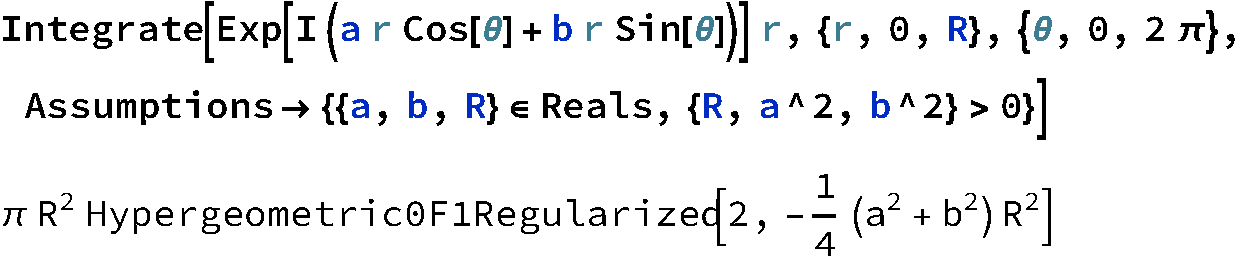
\includegraphics[width=\textwidth]{nasty-integral.pdf}
  
  
  
  \chapter{Simplification of Equation \ref{eq:expected_refl} Given Normal Light Incidence}\label{chap:airy_validation}
  
  Simplification was done with Mathematica 13.1.0.
  
  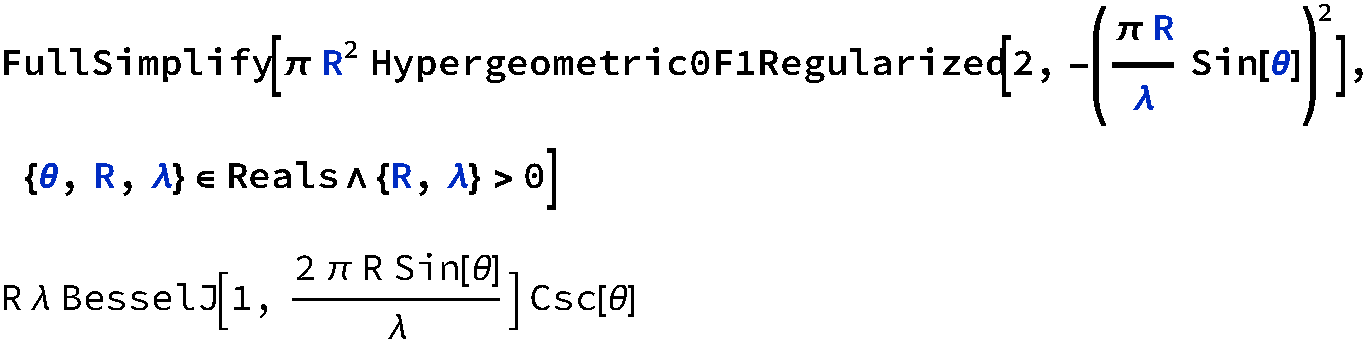
\includegraphics[width=\textwidth]{airy-simplification.pdf}
  
\end{appendices}

%%%%%%%%%%%%%%%%%%%%%%%%%%%%%%%%%%%%%%%%%%%%%%%%%%%%%%%%%%%%%%%%%%%%%%%%%%%%%%%%%%%%%%%%%%%%%%%%%%%%%%%%%%%%%%%%%%%%%%%%





% Make the bibliography.
% Enter your references in the BibTex file "references.bib"
\bibliography{references}

% Make the index
\printindex

\end{document}
